\chapter{Kết quả kiểm định}
\label{ch:ketqua}

\section{Hiệu năng tổng thể}

Trên tập test (638 ảnh, 770 đối tượng): Precision = 0,960, Recall = 0,951, mAP@0,5 = 0,970,
mAP@0,5:0,95 = 0,812. Trên tập valid, mAP@0,5 = 0,976. Nhìn tổng thể đây là kết quả rất tốt ---
nhưng con số tổng che giấu ba vấn đề mà ba mục sau đây làm rõ.

\section{CH-A --- Rò rỉ dữ liệu}

Chính bước EDA của notebook đã phát hiện trùng lặp bằng perceptual hash và so khớp chính xác. Tuy
nhiên quy trình chỉ loại trùng khỏi tập huấn luyện, còn tập kiểm thử --- vốn dùng để chấm điểm
--- không được khử trùng (Bảng~\ref{tab:leak}, Hình~\ref{fig:leak}).

\begin{table}[H]
\centering
\caption{Trùng lặp và rò rỉ dữ liệu}
\label{tab:leak}
\small
\begin{tabular}{lrr}
\toprule
\textbf{Loại trùng lặp} & \textbf{Số dòng ảnh} & \textbf{\% trên tổng thể} \\
\midrule
Exact duplicate (mọi split) & 460 & 4,63\% \\
Exact duplicate xuyên split & 202 & 2,03\% \\
dHash trùng (mọi split) & 799 & 8,04\% \\
dHash trùng xuyên split & 423 & 4,26\% \\
\bottomrule
\end{tabular}
\end{table}

\begin{figure}[H]
\centering
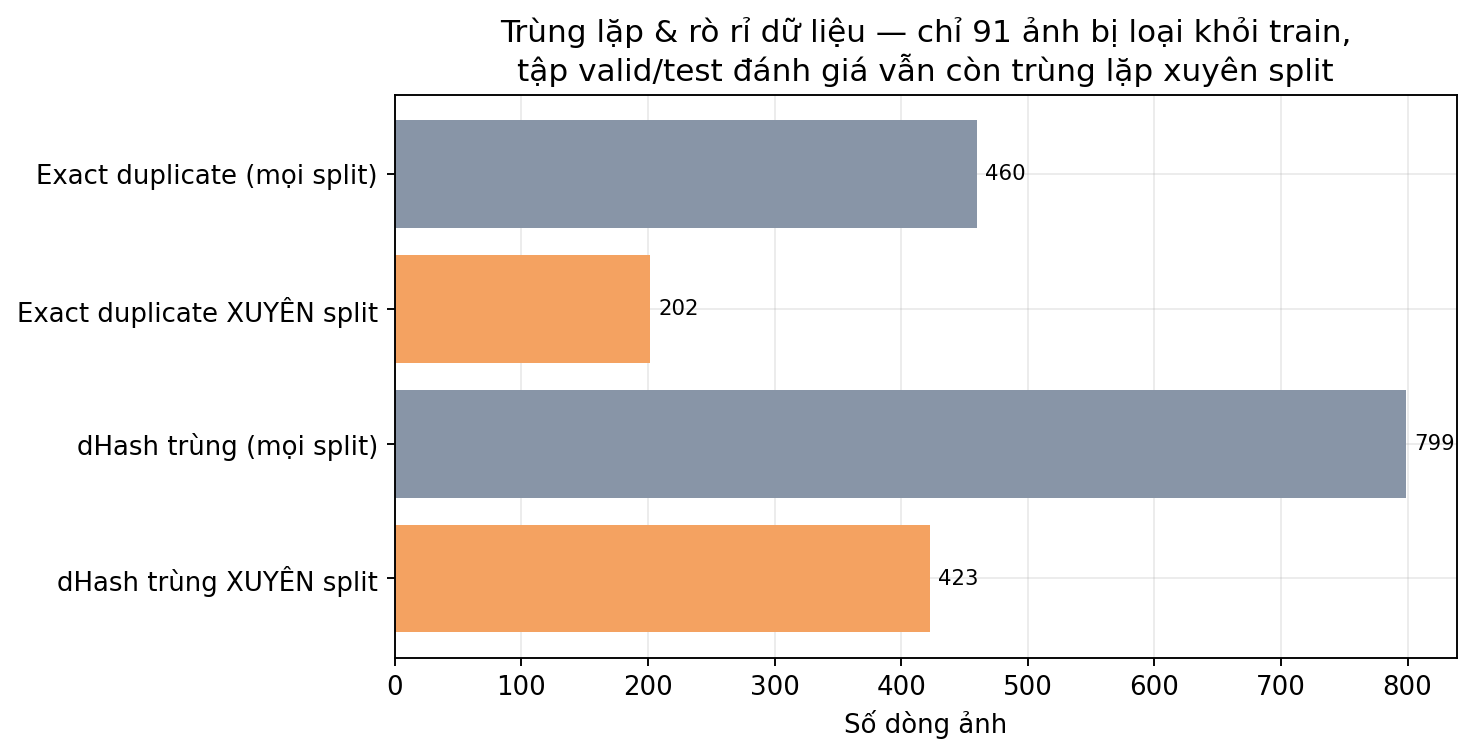
\includegraphics[width=0.82\textwidth]{figures/04_leakage.png}
\caption{Trùng lặp và rò rỉ --- chỉ 91 ảnh bị loại khỏi tập huấn luyện, valid/test vẫn còn trùng}
\label{fig:leak}
\end{figure}

\hopnhanmanh[Nhận xét CH-A]{Notebook chỉ loại 91 ảnh exact-cross-split khỏi tập huấn luyện
($3.530 \to 3.439$). Vẫn còn 202 ảnh trùng chính xác và 423 ảnh gần trùng xuyên split không bị
loại ở tập valid/test. Hệ quả: một phần điểm mAP 0,97 có thể đến từ việc mô hình đã ``thấy'' ảnh
rất giống lúc huấn luyện --- con số thực có thể thấp hơn.}

\section{CH-B --- Khoảng cách đèn tín hiệu và biển báo}

Bảng~\ref{tab:perclass} trình bày hiệu năng theo từng lớp, sắp xếp giảm dần theo mAP@0,5:0,95.

\begin{table}[H]
\centering
\caption{Hiệu năng theo lớp trên tập test}
\label{tab:perclass}
\small
\begin{tabular}{llrrrrr}
\toprule
\textbf{Lớp} & \textbf{Nhóm} & \textbf{Inst.} & \textbf{P} & \textbf{R} & \textbf{mAP@.5}
& \textbf{mAP@.5:.95} \\
\midrule
Stop & Biển báo & 50 & 0,999 & 1,000 & 0,995 & 0,899 \\
Speed Limit 80 & Biển báo & 61 & 0,977 & 1,000 & 0,995 & 0,878 \\
Speed Limit 100 & Biển báo & 46 & 0,968 & 1,000 & 0,994 & 0,871 \\
Speed Limit 70 & Biển báo & 53 & 0,922 & 0,943 & 0,973 & 0,867 \\
Speed Limit 20 & Biển báo & 46 & 0,972 & 0,978 & 0,973 & 0,866 \\
Speed Limit 120 & Biển báo & 44 & 0,930 & 1,000 & 0,985 & 0,863 \\
Speed Limit 30 & Biển báo & 60 & 0,983 & 0,966 & 0,984 & 0,860 \\
Speed Limit 60 & Biển báo & 45 & 1,000 & 0,933 & 0,992 & 0,859 \\
Speed Limit 50 & Biển báo & 50 & 0,928 & 0,960 & 0,987 & 0,856 \\
Speed Limit 40 & Biển báo & 53 & 0,977 & 0,962 & 0,982 & 0,838 \\
Speed Limit 10 & Biển báo & 3 & 1,000 & 0,971 & 0,995 & 0,830 \\
Speed Limit 90 & Biển báo & 34 & 0,995 & 0,971 & 0,993 & 0,827 \\
Speed Limit 110 & Biển báo & 21 & 0,906 & 0,905 & 0,930 & 0,784 \\
\textbf{Green Light} & \textbf{Đèn} & 110 & 0,962 & 0,921 & 0,950 & \textbf{0,576} \\
\textbf{Red Light} & \textbf{Đèn} & 94 & 0,887 & 0,755 & 0,825 & \textbf{0,506} \\
\bottomrule
\end{tabular}
\end{table}

\begin{figure}[H]
\centering
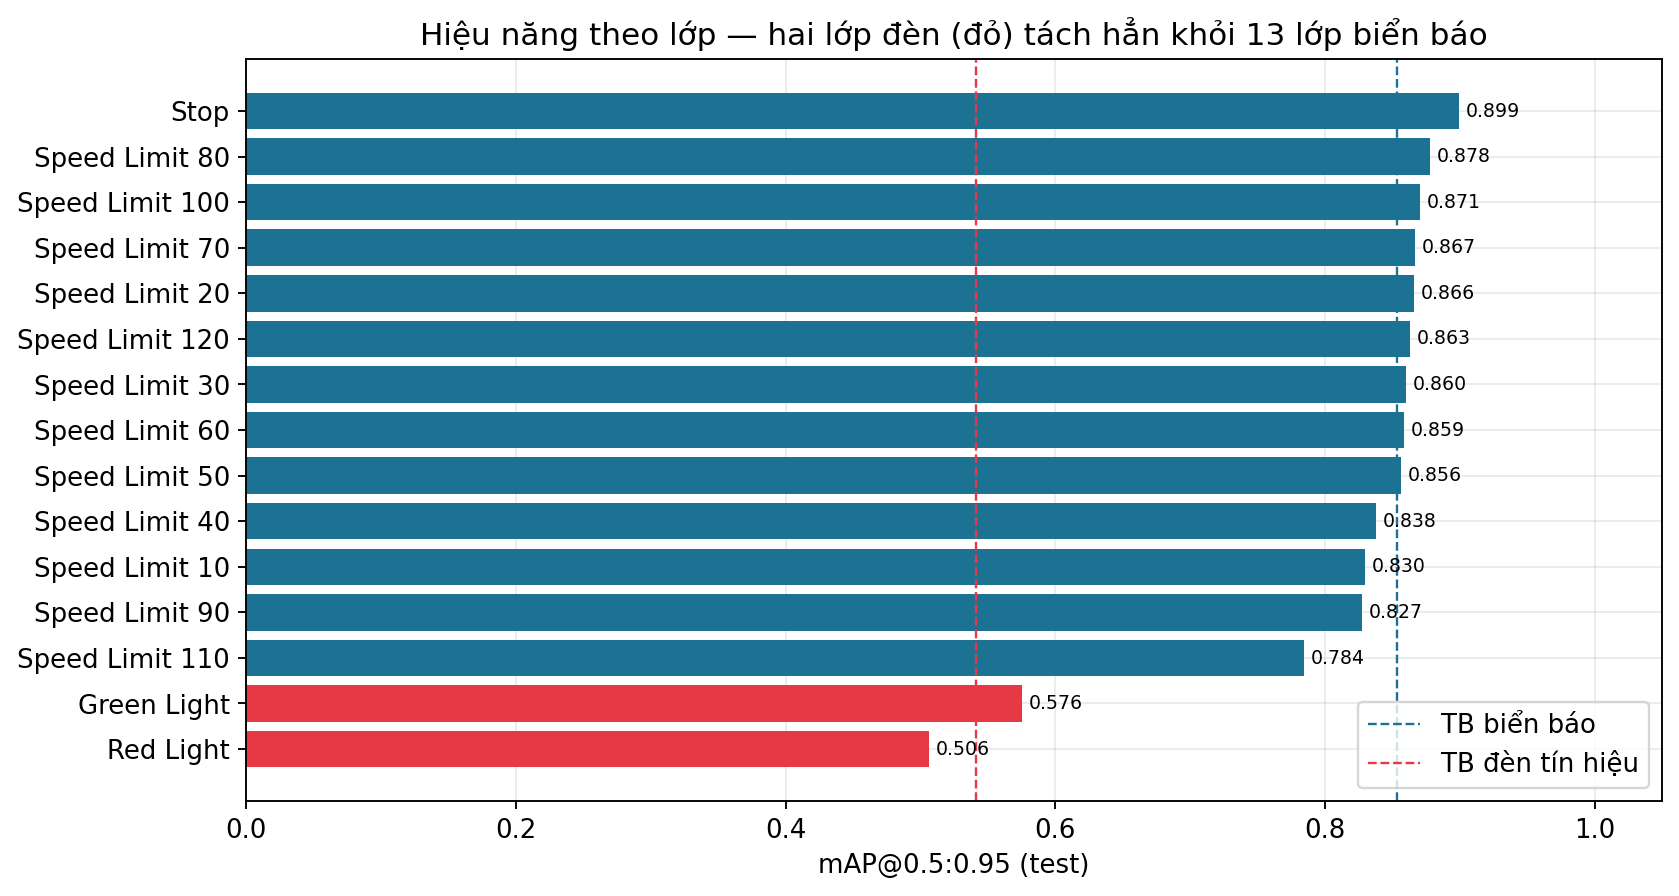
\includegraphics[width=0.92\textwidth]{figures/01_per_class_ap.png}
\caption{Hiệu năng theo lớp --- hai lớp đèn (đỏ) tách hẳn khỏi 13 lớp biển báo}
\label{fig:perclass}
\end{figure}

\begin{figure}[H]
\centering
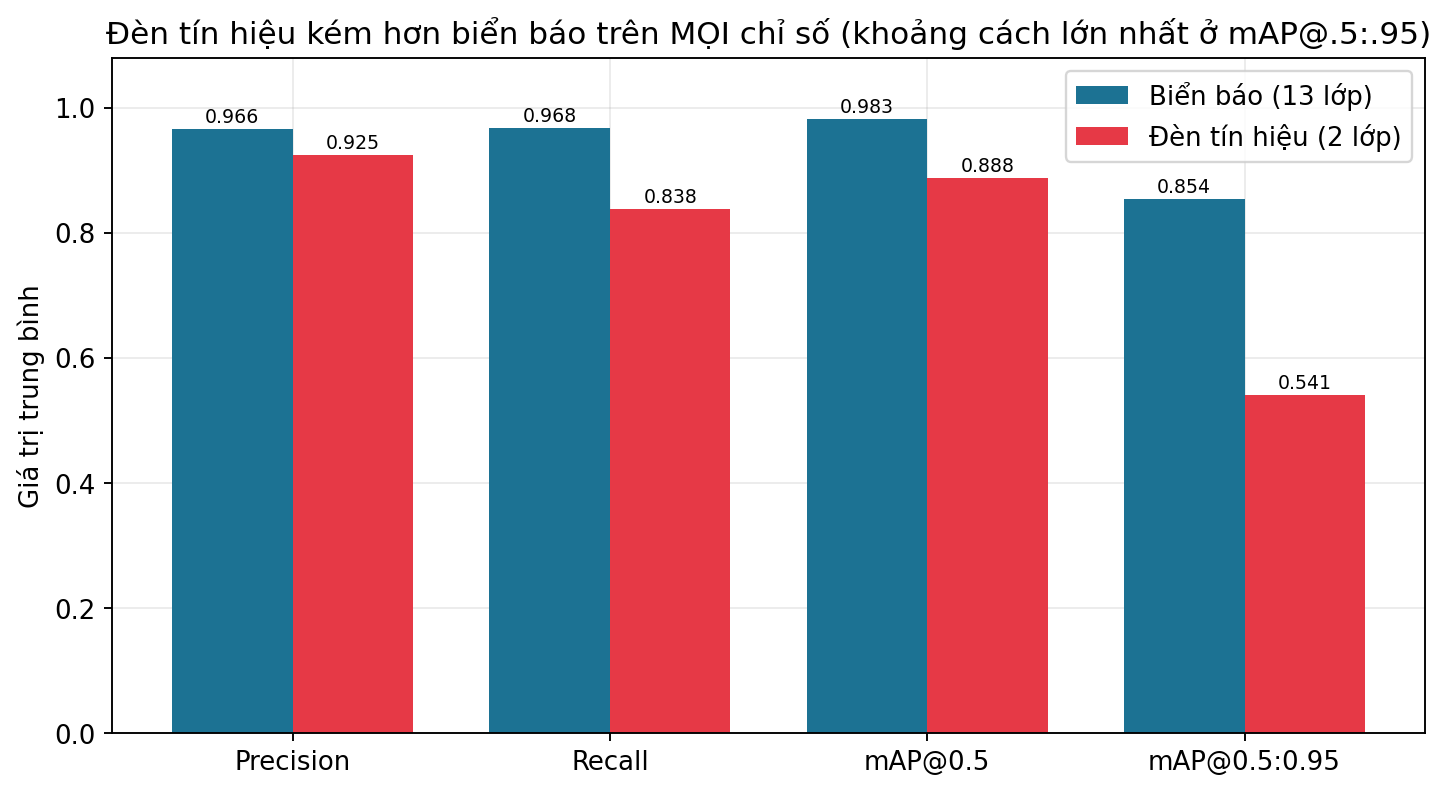
\includegraphics[width=0.82\textwidth]{figures/02_light_vs_sign.png}
\caption{Đèn tín hiệu kém hơn biển báo trên mọi chỉ số}
\label{fig:lightsign}
\end{figure}

\hopnhanmanh[Nhận xét CH-B]{Trung bình mAP@0,5:0,95: đèn tín hiệu 0,541 so với biển báo 0,854 ---
chênh 0,313. Kiểm định Mann--Whitney một phía cho $p = 0{,}0095$: khác biệt có ý nghĩa dù chỉ có
2 lớp đèn. Red Light là lớp kém nhất (mAP@0,5:0,95 = 0,506; recall chỉ 0,755).}

\section{CH-C --- Hiếm không đồng nghĩa với khó}

Một giả thuyết tự nhiên là ``đèn kém vì hiếm''. Bằng chứng bác bỏ điều này: tương quan Spearman
giữa số đối tượng trên test và mAP@0,5:0,95 là $\rho = 0{,}032$ ($p = 0{,}91$) --- gần như bằng
0 (Hình~\ref{fig:rarity}). Ngược lại, hai lớp có \emph{nhiều} đối tượng nhất trên tập test
(Green Light 110 và Red Light 94 đối tượng) lại rơi đúng vào nhóm kém nhất.

\begin{figure}[H]
\centering
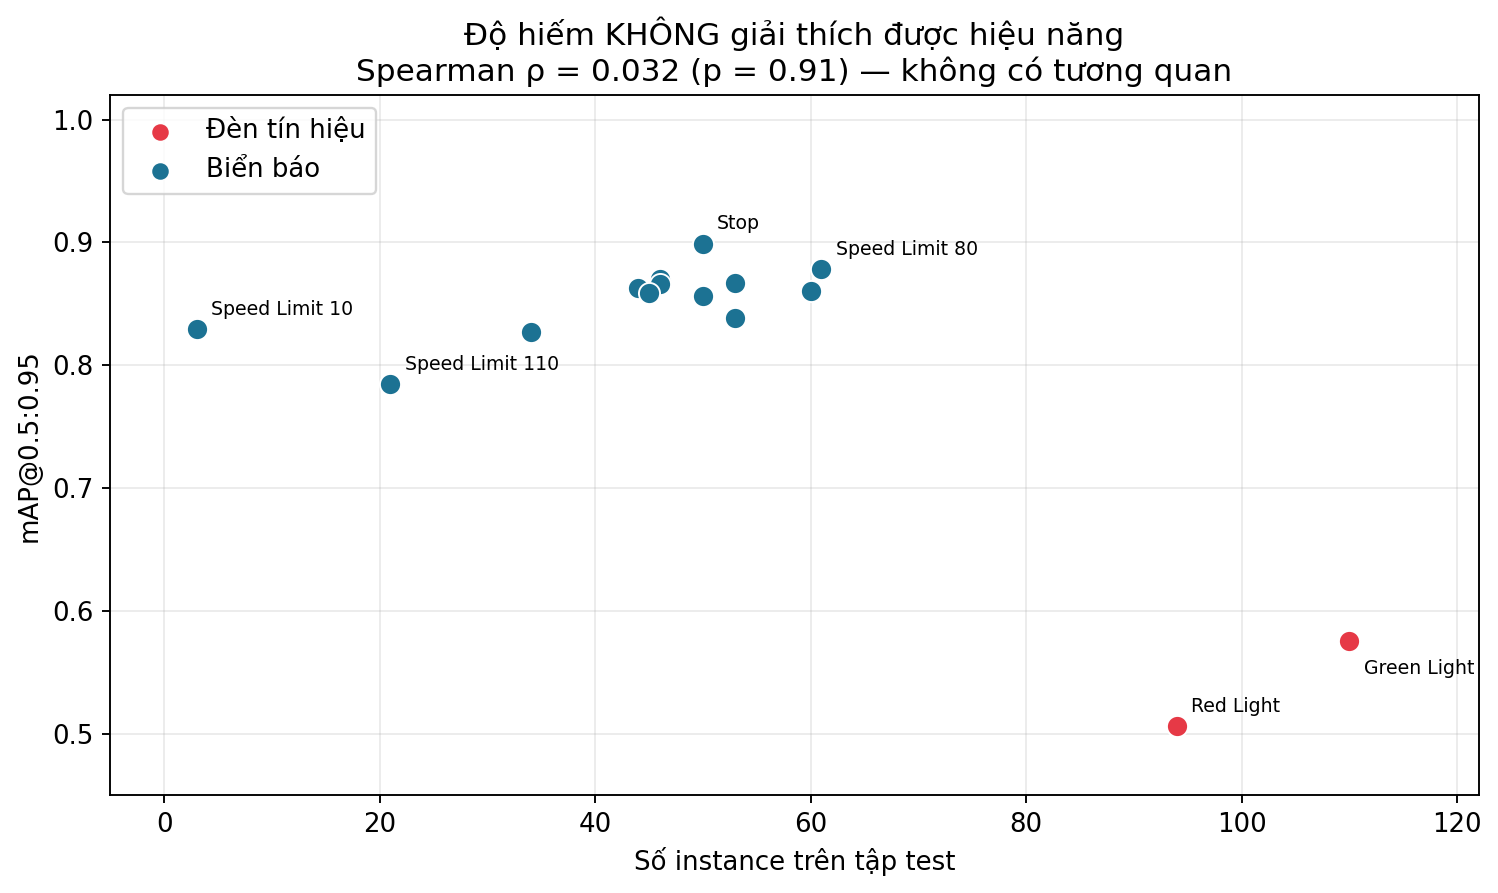
\includegraphics[width=0.82\textwidth]{figures/03_rarity_vs_ap.png}
\caption{Độ hiếm không giải thích được hiệu năng ($\rho \approx 0$)}
\label{fig:rarity}
\end{figure}

\hopnhanmanh[Nhận xét CH-C]{Độ hiếm của lớp không dự báo được hiệu năng --- mất cân bằng không
phải nguyên nhân. Nguyên nhân nằm ở bản chất vật thể: đèn tín hiệu thường nhỏ, độ tương phản
thấp, và hai màu đỏ/xanh dễ nhầm về hình học. Bối cảnh kích thước: 36,6\% đối tượng là ``nhỏ''
($<1\%$ diện tích ảnh) và 18,7\% là ``tí hon'' ($<0{,}1\%$).}

\section{Mất cân bằng và kích thước --- bối cảnh}

Toàn corpus có tỉ số mất cân bằng 35,8, entropy chuẩn hoá 0,953 và hệ số Gini 0,247 --- mất cân
bằng mức trung bình (Hình~\ref{fig:imb}). Độ dịch phân phối giữa các split rất nhỏ (Jensen--Shannon
$\le 0{,}008$ bit), nên chênh lệch hiệu năng không đến từ việc phân phối lớp khác nhau giữa các
tập. Về kích thước, tăng độ phân giải đầu vào làm giảm mạnh tỉ lệ vật thể tí hon
(Hình~\ref{fig:size}) --- cơ sở cho khuyến nghị tăng \texttt{imgsz} ở Chương~\ref{ch:tongket}.

\begin{figure}[H]
\centering
\begin{subfigure}{0.48\textwidth}
  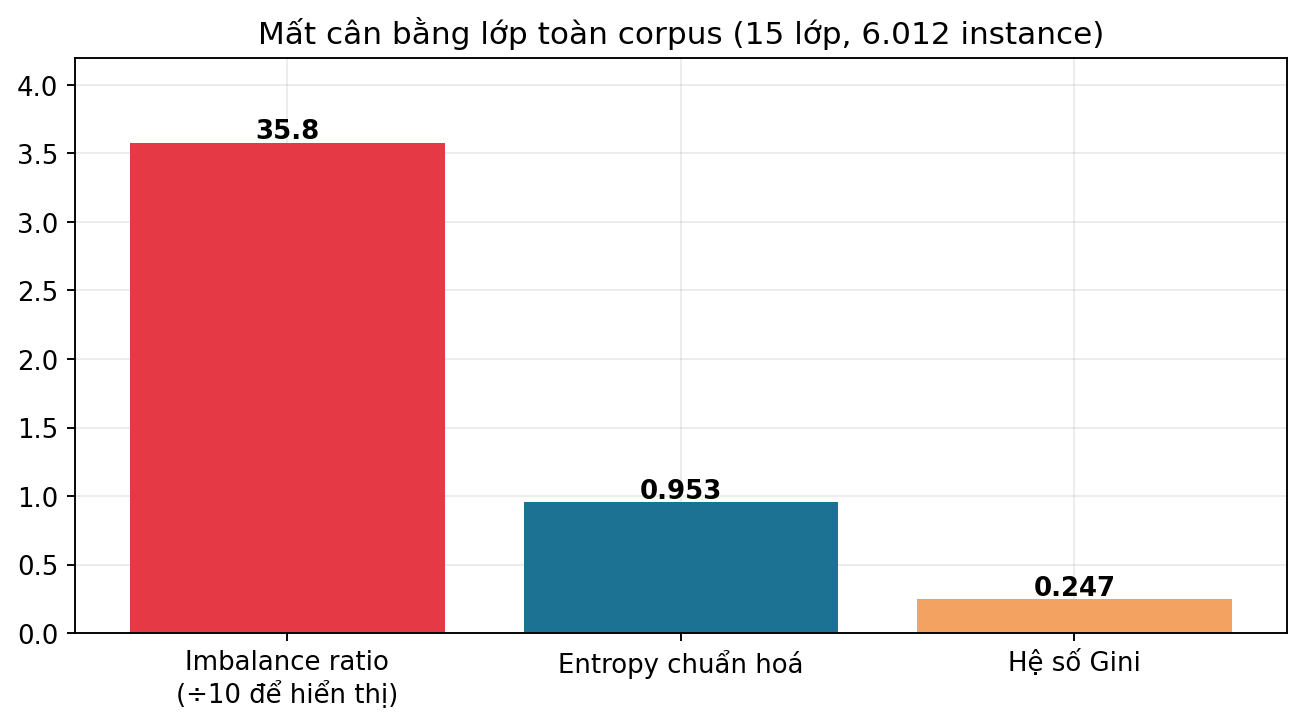
\includegraphics[width=\linewidth]{figures/05_imbalance.png}
  \caption{Mất cân bằng lớp}
  \label{fig:imb}
\end{subfigure}\hfill
\begin{subfigure}{0.48\textwidth}
  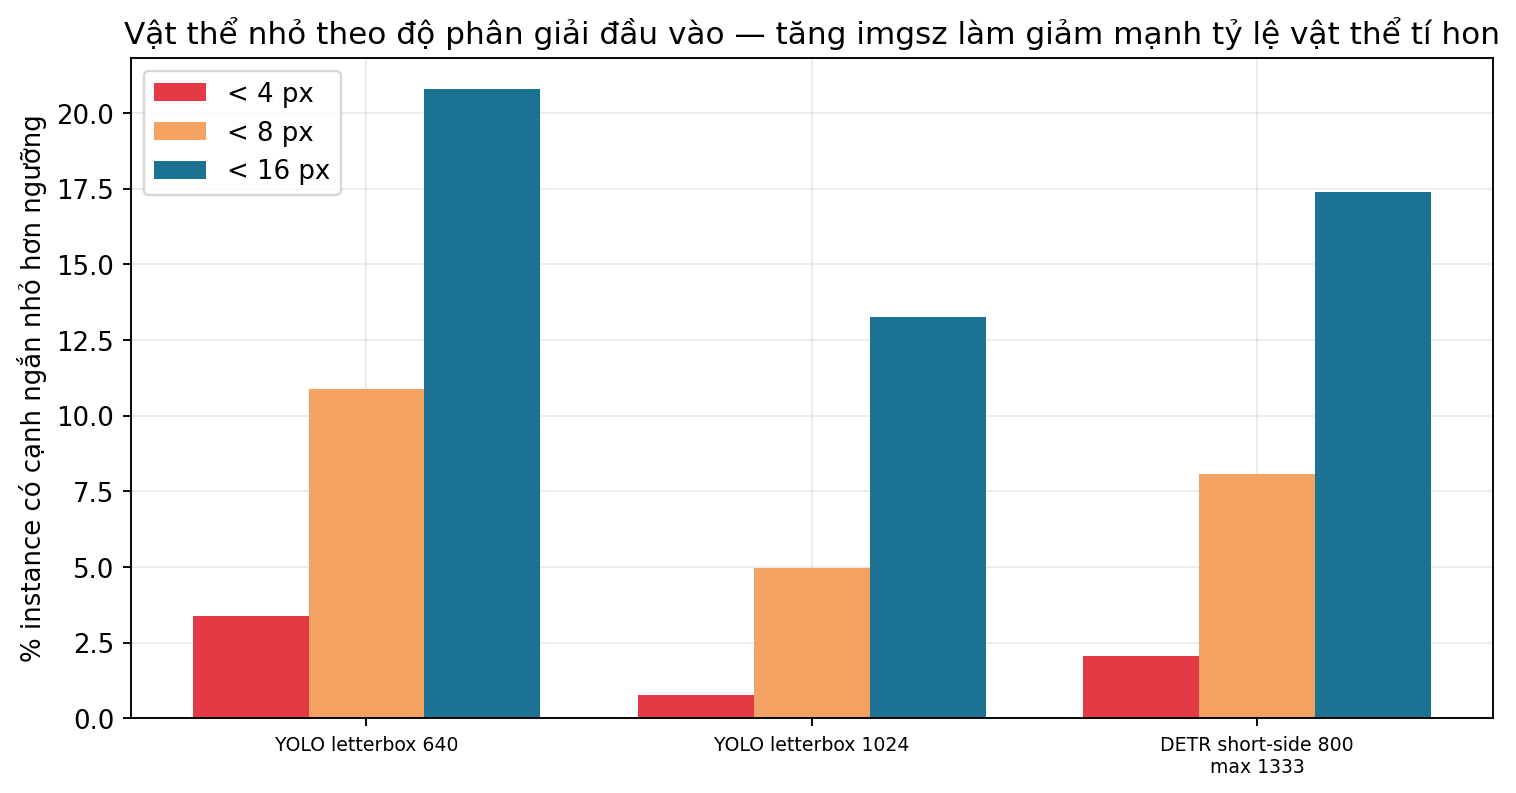
\includegraphics[width=\linewidth]{figures/06_small_objects.png}
  \caption{Vật thể nhỏ theo độ phân giải}
  \label{fig:size}
\end{subfigure}
\caption{Bối cảnh mất cân bằng (trái) và kích thước vật thể (phải)}
\label{fig:context}
\end{figure}
